\section{ED-EMS application}\label{sec:queueing_ems_es_application}

The queueing network described in Section~\ref{sec:queueing_section} can be
directly applied to a healthcare setting.
The healthcare scenario that is of interest here is at the interface between
Emergency Department (ED) staff and Emergency Medical Services (EMS) staff.
All parameters described in Section~\ref{sec:queueing_section} can be mapped
to some components of either the ED or the EMS.

\begin{itemize}
    \item \(\lambda_1 \rightarrow\) Type 1 individuals \(\rightarrow\)
    Individuals arriving without an ambulance (or via an ambulance that cannot
    be blocked)
    \item \(\lambda_2 \rightarrow\) Type 2 individuals \(\rightarrow\)
    Individuals arriving with an ambulance (that can be blocked)
    \item \(\mu \rightarrow\) Service rate \(\rightarrow\) The service rate of a
    patient
    \item \(C \rightarrow\) Number of servers \(\rightarrow\) The number of
    beds in the hospital
    \item \(T \rightarrow\) Threshold \(\rightarrow\) The number of patients that
    need to be in the hospital to start blocking ambulances in the parking area.
    \item \(N \rightarrow\) Node 1 capacity \(\rightarrow\) The overall hospital
    capacity (i.e. the number of beds in the hospital plus the queueing
    capacity)
    \item \(M \rightarrow\) Node 2 capacity \(\rightarrow\) The parking capacity
\end{itemize}

Type 1 individuals are now all patients that arrive at the ED via
some other means of transportation rather than an ambulance.
Type 2 individuals are now all patients that arrive at the ED via an ambulance
whose condition allows them to be delayed in the parking lot.
The threshold parameter \(T\) is now the amount of patients that need to be in
the hospital waiting area (and in service) to start blocking ambulances in the
parking area.
Figure~\ref{fig:diagram_of_queueing_system_applied_to_ed_ems} shows the applied
version of Figure~\ref{fig:diagram_of_queueing_system} that is the queueing
network introduced in Section~\ref{sec:queueing_section}.

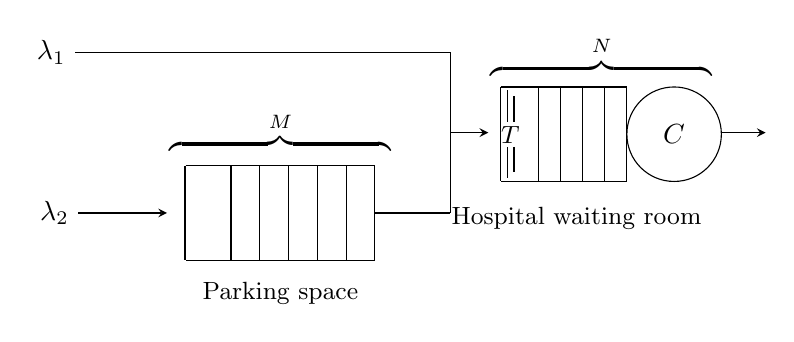
\begin{tikzpicture}[>=stealth, scale=0.8],
    % the rectangle of Queue 1
    \draw (0,0) -- ++(3cm,0) -- ++(0,-1.5cm) -- ++(-3cm,0);
    % The label above Queue 1 -> M
    \node[anchor=north] at (1.5cm, 1cm) {\(
        \overbrace{\qquad \qquad \qquad \qquad}^{M}
    \)};
    % The label below Queue 1 -> Waiting zone 2
    \node[anchor=north] at (1.5cm, -1.7cm) {\small{Parking space}};

    % the vertical lines in Queue 1
    \foreach \i in {1,...,5, 6.6}
    \draw (3cm-\i*13pt,0) -- +(0,-1.5cm);

    % % the circle in Queue 1
    % \draw (2.75,-0.75cm) circle [radius=0.75cm] node {\(0\)};

    % the rectangle in Queue 2
    \draw (5,1.25) -- ++(2cm,0) -- ++(0,-1.5cm) -- ++(-2cm,0);
    % the vertical lines in Queue 2
    \foreach \i in {1,...,4, 5.7}
    \draw (7cm-\i*10pt,1.25) -- +(0,-1.5cm);
    % The two vertical lines at the start of Queue 2
    \draw (7cm-54pt,1.2) -- +(0,-0.5cm);
    \draw (7cm-54pt,0.3) -- +(0,-0.5cm);
    \draw (7cm-51pt,1.1) -- +(0,-0.4cm);
    \draw (7cm-51pt,0.3) -- +(0,-0.4cm);

    % The label between the lines for T
    \node[anchor=north] at (5.15, 0.77 cm) {\small{\( T \)}};

    % The label above Queue 2 -> N
    \node[anchor=north] at (6.6cm, 2.2cm) {\(
        \overbrace{\qquad \qquad \qquad \qquad}^{N}
    \)};
    % The label below Queue 2 -> Waiting zone 1
    \node[anchor=north] at (6.2cm, -0.5cm) {\small{Hospital waiting room}};

    % the circle in Queue 2
    \draw (7.75,0.5) circle [radius=0.75cm] node {\(C\)};

    % Arrow line from Queue 2 outside
    \draw[->] (8.5,0.525) -- +(20pt,0);

    % Line from lambda_2 to Queue 1
    \draw[<-] (-0.3,-0.75) -- +(-40pt,0) node[left] {\( \lambda_2 \)};
    % First line (horizontal) after Queue 1
    \draw[-] (3,-0.75) -- +(34pt,0);
    % Second line (vertical) after Queue 1
    \draw (4.2, 0.525) -- (4.2, -0.75);

    % First line (horizontal) from lambda_1
    \draw (4.2, 1.8) -- +(-169.5pt,0) node[left] {\( \lambda_1 \)};
    % Second line (vertical) from lambda_1
    \draw (4.2, 1.8) -- (4.2, 0.525);
    % Arrow line to Queue 2
    \draw[->] (4.2, 0.525) -- (4.8, 0.525);
\end{tikzpicture}


The performance measures of the queueing system
have an additional meaning under the context of this new application.
The average number of individuals in Node 1 and Node 2 are now the average
number of patients in the hospital and the average number of ambulances in the
parking space.
The mean waiting time of individuals described in Section~\ref{sec:waiting_time}
is the average waiting time patients wait in Node 1 before they are seen by a
doctor or nurse.
Similarly, the mean blocking time from Section~\ref{sec:blocking_time}
is the mean time ambulances stay blocked in the parking space before the
individuals they carry are allowed to enter the hospital.
Finally, the proportion of individuals whose waiting time is longer than a
predefined target time, described in
Section~\ref{sec:proportion_of_individuals_within_time}
is now the percentage of patients that wait longer than a predefined time
before they are seen by a doctor or nurse.